\documentclass[14pt]{extarticle}
\usepackage{amsmath}
\usepackage{amssymb}
\usepackage{graphicx}
\graphicspath{ {../chap09/} }
\usepackage[top=1in, bottom=0.75in, left=0.75in, right=0.75in]{geometry}
\newcommand*{\Scale}[2][4]{\scalebox{#1}{\ensuremath{#2}}}%
\usepackage{hyperref}


\begin{document}

\section*{Math208 Discussion Outline for 11/05/2020}

\subsection{Homework and other due dates}
\begin{itemize}
\item Section 9.4 - 9.5 due 11/6
\item Section 9.5 due 11/10
\item Complete the Instruction Survey
\item In class assignment due 11/8 \\\\
\resizebox{12cm}{!}{
	{A photo that has meaning to you}
}
\end{itemize}

\subsection{Questions?}
\begin{itemize}
	\item I posted videos for some 9.2 and 9.4 questions
\end{itemize}

\subsection{Goals}
\subsubsection*{Section 9.4: The Derivative and Section 9.5: Differentiation}
\begin{itemize}
	\item Understand the meaning and interpretations of the derivative
	\item Use the four-step process to find the derivative from its definition
	\item Use Differentiation Properties to find the derivative.
\end{itemize}

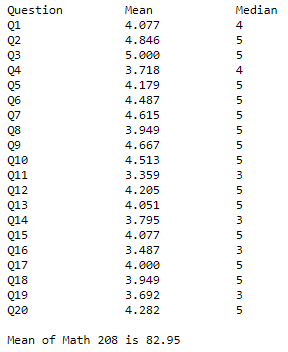
\includegraphics[width=0.4\linewidth]{exam2-results}



\cleardoublepage



\subsection*{Section 9.4: The Derivative}
\subsubsection*{Some Graphs}
\begin{itemize}
	\item X-limits, \url{https://www.desmos.com/calculator/vshkxi2kdb}
	\item Secant line to tangent line, \url{https://www.desmos.com/calculator/faudtsxdzy}
	\item Distance-velocity-accelerate, \url{https://www.desmos.com/calculator/jgxmedmm8n}
\end{itemize}
\subsubsection*{The Derivative}
\begin{center}
	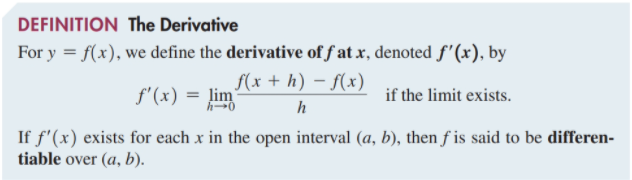
\includegraphics[width=0.95\linewidth]{9-4-1} \\
	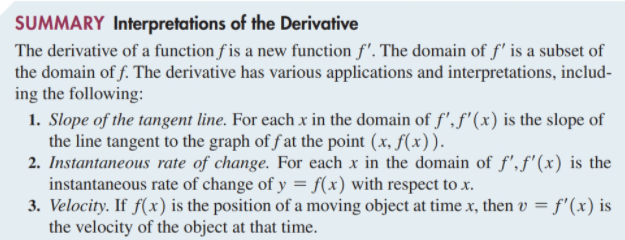
\includegraphics[width=0.95\linewidth]{9-4-2} \\
	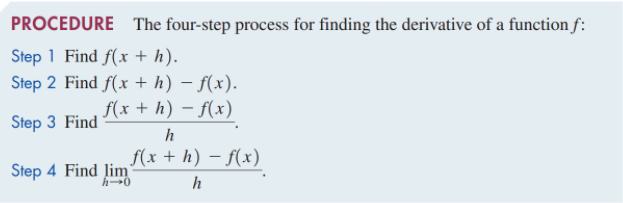
\includegraphics[width=0.95\linewidth]{9-4-3} \\
\end{center}

\cleardoublepage

\subsection*{Section 9.5: Differentiation}
\begin{center}
	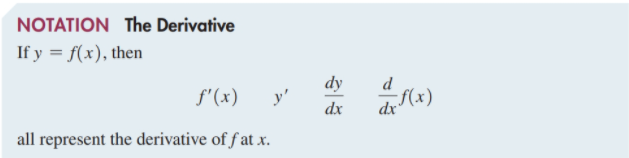
\includegraphics[width=0.8\linewidth]{9-5-1} \\
	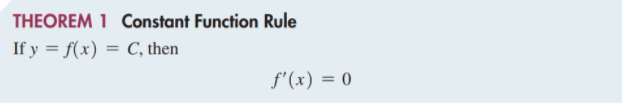
\includegraphics[width=0.8\linewidth]{9-5-2} \\
	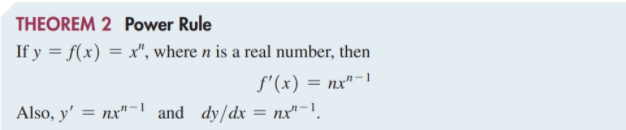
\includegraphics[width=0.8\linewidth]{9-5-3} \\
	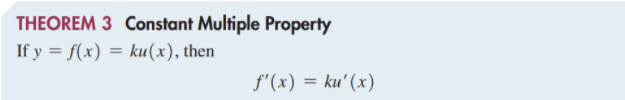
\includegraphics[width=0.8\linewidth]{9-5-4} \\
	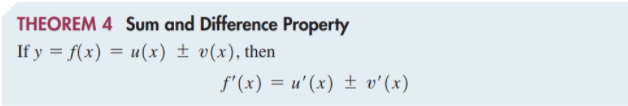
\includegraphics[width=0.8\linewidth]{9-5-5} \\
	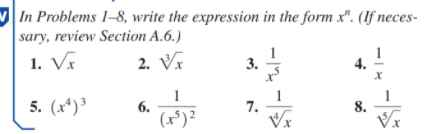
\includegraphics[width=0.8\linewidth]{9-5-6a} \\
\end{center}
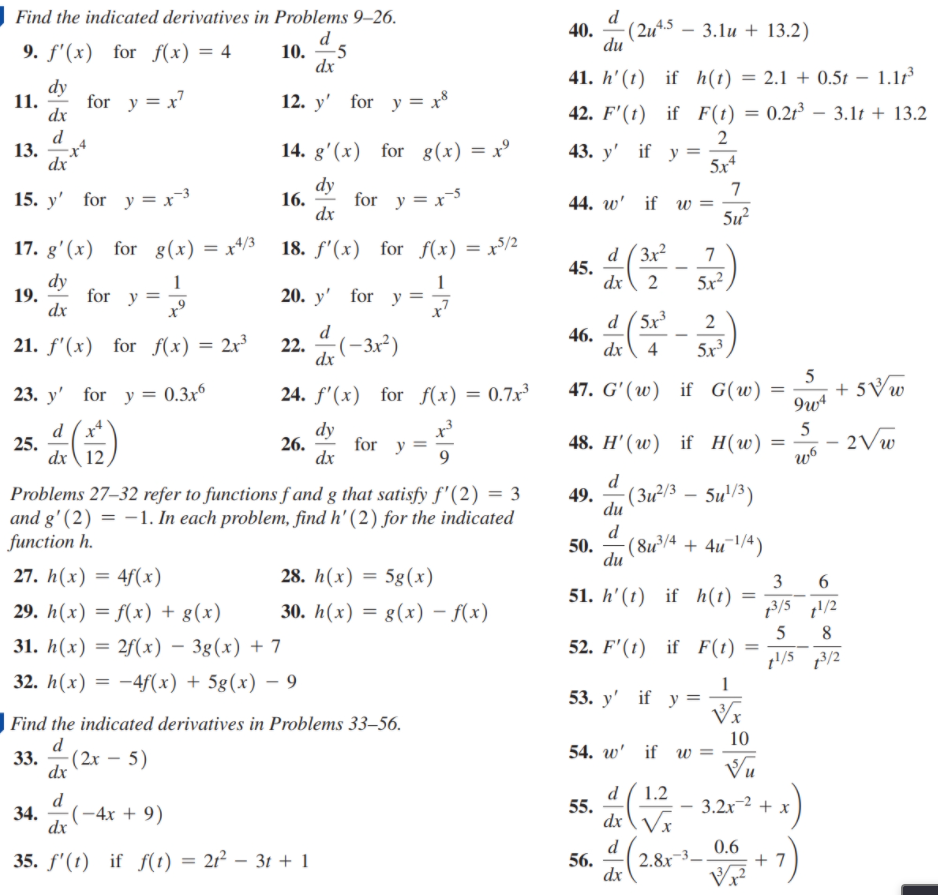
\includegraphics[width=1.1\linewidth]{9-5-7}
\\
\textbf{Application}: Say the velocity (in miles/hour) of a car is given by:
\begin{align*}
v(t)=-2t^2 + 20t
\end{align*}
What is the maximum velocity of the car? (in other words, What is the maximum of this parabola?)







\end{document}
